\documentclass[letterpaper, 10pt, conference, twoside]{ieeeconf}


\IEEEoverridecommandlockouts
\overrideIEEEmargins
\usepackage{ctex}
\usepackage{booktabs}
\usepackage{graphicx}
\graphicspath{{figures/}}%图片所在的目录

\usepackage{lastpage}%获得总页数
\usepackage{fancyhdr}
\pagestyle{fancy}
%以下命令中L--左侧 R--右侧 C--中间 O--奇数页 E--偶数页
%\fancyhead[LO,RE]{机器学习原理、工程技术与应用}%奇数页左侧,偶数页右侧显示页眉
\fancyhead[CO,RE]{机器学习}%奇数页左侧,偶数页右侧显示页眉
\fancyhead[LO,CE]{代课教师 李乡儒,华南师范大学计算机学院}%奇数页左侧,偶数页中间页脚为空
\fancyhead[RO,LE]{\today}%奇数页右侧,偶数页左侧显示 当前页 of 总页数
\fancyfoot[CO,RE]{机器学习}%奇数页中间,偶数页右侧页脚为空
\fancyfoot[LO,CE]{2021-2022-2学期}%奇数页左侧,偶数页中间页脚为空
\fancyfoot[RO,LE]{\thepage\ of \pageref{LastPage}}%奇数页右侧,偶数页左侧显示 当前页 of 总页数
\renewcommand{\headrulewidth}{0.4pt}%改为0pt即可去掉页眉下面的横线
\renewcommand{\footrulewidth}{0.4pt}%改为0pt即可去掉页脚上面的横线
\setlength{\voffset}{-10mm}
\setlength{\topmargin}{0mm}
\setlength{\headheight}{5mm}
\setlength{\headsep}{5mm}
\setlength{\footskip}{8mm}



\title{\LARGE \bf
基于U-Net的胃肠道图像分割
}


\author{2021023206 \quad 徐力\\ \today\\ 机器学习课程作业}


\begin{document}

\maketitle
%\thispagestyle{empty}
%\pagestyle{empty}



\begin{abstract}
该模板适用于机器学习高级技术及应用课程. 所有地方使用英文状态下的标点符号, 标点符号之后空一个空格.

\vspace{1ex}\noindent\textbf{关键词}: 词1; 词2

\end{abstract}

\begin{eabstract}
	English Abstract
	
\vspace{1ex}\noindent\textbf{Keywords}: word1; word2
\end{eabstract}


\section{引言}
医学图像分割是医学图像处理与分析领域的复杂而关键的步骤,其目的是将医学图像中具有某些特殊含义的部分分割出来,并提取相关特征,为临床诊疗和病理学研究提供可靠的依据,辅助医生作出更为准确的诊断。 医学图像具有复杂性,在分割过程中需要解决不均匀及个体差异等一系列问题,所以一般的图像分割方法难以直接应用于医学图像分割。

UW-Madison 胃肠道图像分割(UW-Madison GI Tract Image Segmentation)是一场研究型代码竞赛,要求在医学扫描中跟踪健康肠胃器官的准确位置以改善肠胃癌的放射治疗。在治疗当中,借助集成磁共振成像和线性加速器系统(也称为 MR-Linacs)等技术,为了指向肿瘤施加高剂量辐射,同时避开肠和胃,放射肿瘤学家必须手动勾勒出胃和肠的位置。这项工作非常耗时,因为肿瘤、肠和胃的位置每天都在变化,使得治疗时间大大延长。

在比赛中,需要创建模型以在MRI扫描中自动分割肠和胃。在给出的数据集中,不同的患者在不同日子里进行了多次MRI扫描,每次扫描包括多张断层扫描。
% \subsection{二级标题}
% \subsubsection{三级标题}

\section{U-Net框架}
U-Net 的构建基于“全卷积网络”。它由收缩路径(左侧)和扩展路径(右侧)组成。收缩路径遵循卷积网络的典型架构。它由两个 3x3 卷积(未填充卷积)的重复应用组成,每个卷积后跟一个整流线性单元 (ReLU) 和一个 2x2 最大池化操作,步幅为 2,用于下采样。在每个下采样步骤中,我们将特征通道的数量加倍。扩展路径中的每一步都包括对特征图进行上采样,然后是将特征通道数量减半的 2x2 卷积(“上卷积”),与收缩路径中相应裁剪的特征图的连接,以及两个 3x3卷积,每个后跟一个 ReLU。由于在每个卷积中都会丢失边界像素,因此裁剪是必要的。在最后一层,使用 1x1 卷积将每个 64 分量特征向量映射到所需数量的类。该网络总共有 23 个卷积层,如图 1 所示。
\begin{figure}[htbp]
  \centering
  \includegraphics[width = 1\linewidth]{structure.png}
  \caption{U-Net 结构}
  \label{fig:fig1}
\end{figure}

在上采样部分,上采样的特征图包含了上下文信息,并与来自收缩路径的高分辨率特征结合,将上下文信息传播到更高分辨率的层。分割图只包含输入图像中完整上下文可用的像素,为了预测图像边界区域中的像素,通过镜像输入图像来推断缺失的上下文,如图2所示。

\begin{figure}[htbp]
  \centering
  \includegraphics[width = 1\linewidth]{seamless-seg.png}
  \caption{U-Net 结构}
  \label{fig:fig2}
\end{figure}

生物医学图像分割中,可用的训练数据通常较少。因此,需要对可用的训练图像应用数据增强,如弹性变形等。这允许网络学习对此类变形的不变性。同时在生物医学当中,变形曾经是组织中最常见的变化,并且可以有效地模拟真实的变形。通过数据增强,模型学习数据的不变性特征,从而防止过拟合。


\section{赛题数据分析}

在本次比赛中,我们在图像中分割器官细胞。训练注释以 RLE 编码掩码的形式提供,图像为 16 位灰度 PNG 格式。

本次比赛中的每个案例都由多组扫描切片表示(每组由扫描发生的日期标识)。有些案例是按时间拆分的(早期是在训练中,后期是在测试中),而有些案例是按案例拆分的——整个案例都在训练中或测试中。本次比赛的目标是能够推广到部分和完全未见的案例。

请注意,在这种情况下,测试集是完全看不见的。如训练集中所示,大约有 50 个案例,具有不同的天数和切片数。



\subsection{二级标题}
\subsubsection{三级标题}

\section{实验}
\subsection{二级标题}
\subsubsection{三级标题}

\section{结论}
\subsection{二级标题}
\subsubsection{三级标题}

\section{图表}

\begin{figure}[htbp]
  \centering
  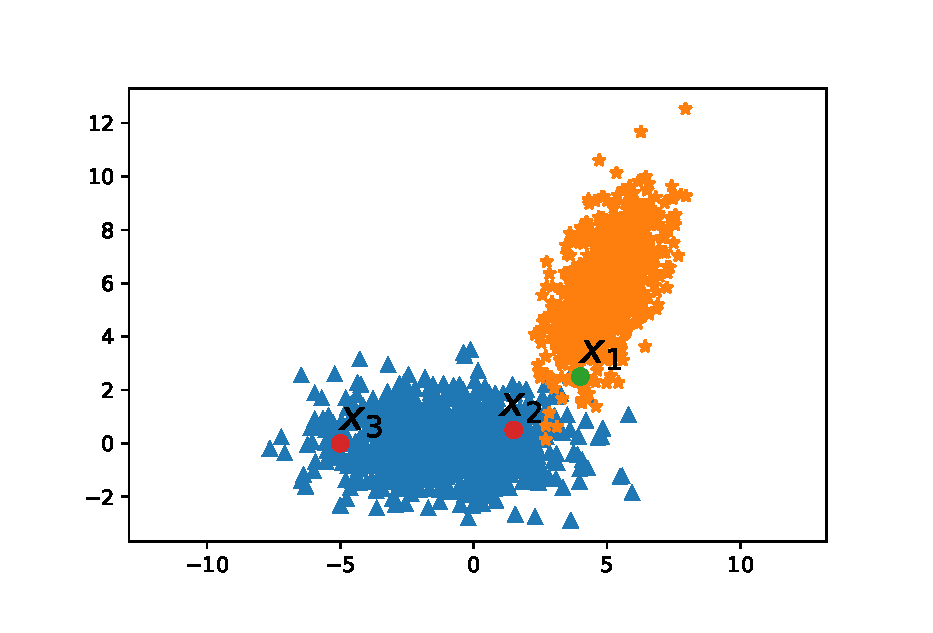
\includegraphics[width = 1\linewidth]{smooth}
  \caption{图片名称及图片内容简介}
  \label{fig:fig2}
\end{figure}


\begin{table}[htbp]
  \centering
 \caption{三线表}
 \label{tab:table2}
 \begin{tabular}{llll}
  \toprule
  表头1 & 表头2 & 表头3& 表头4\\
  \midrule
    模&式&识&别\\
    机&器&学&习\\
    数&据&挖&掘\\
    人&工&智&能\\
  \bottomrule
 \end{tabular}
\end{table}




\section{列点}

\begin{itemize}
\item The word ÒdataÓ is plural, not singular.
\item The subscript for the permeability of vacuum ?0, and other common scientific constants, is zero with subscript formatting, not a lowercase letter ÒoÓ.
\end{itemize}

\begin{enumerate}
\item The word ÒdataÓ is plural, not singular.
\item The subscript for the permeability of vacuum ?0, and other common scientific constants, is zero with subscript formatting, not a lowercase letter ÒoÓ.
\end{enumerate}


\section{脚注}
机器学习\footnote{脚注内容}

\section{列点}

\begin{itemize}
\item The word ÒdataÓ is plural, not singular.
\item The subscript for the permeability of vacuum ?0, and other common scientific constants, is zero with subscript formatting, not a lowercase letter ÒoÓ.
\end{itemize}

\begin{enumerate}
\item The word ÒdataÓ is plural, not singular.
\item The subscript for the permeability of vacuum ?0, and other common scientific constants, is zero with subscript formatting, not a lowercase letter ÒoÓ.
\end{enumerate}


\section{列点}

\begin{itemize}
\item The word ÒdataÓ is plural, not singular.
\item The subscript for the permeability of vacuum ?0, and other common scientific constants, is zero with subscript formatting, not a lowercase letter ÒoÓ.
\end{itemize}

\begin{enumerate}
\item The word ÒdataÓ is plural, not singular.
\item The subscript for the permeability of vacuum ?0, and other common scientific constants, is zero with subscript formatting, not a lowercase letter ÒoÓ.
\end{enumerate}


\section{列点}

\begin{itemize}
\item The word ÒdataÓ is plural, not singular.
\item The subscript for the permeability of vacuum ?0, and other common scientific constants, is zero with subscript formatting, not a lowercase letter ÒoÓ.
\end{itemize}

\begin{enumerate}
\item The word ÒdataÓ is plural, not singular.
\item The subscript for the permeability of vacuum ?0, and other common scientific constants, is zero with subscript formatting, not a lowercase letter ÒoÓ.
\end{enumerate}


\section{列点}

\begin{itemize}
\item The word ÒdataÓ is plural, not singular.
\item The subscript for the permeability of vacuum ?0, and other common scientific constants, is zero with subscript formatting, not a lowercase letter ÒoÓ.
\end{itemize}

\begin{enumerate}
\item The word ÒdataÓ is plural, not singular.
\item The subscript for the permeability of vacuum ?0, and other common scientific constants, is zero with subscript formatting, not a lowercase letter ÒoÓ.
\end{enumerate}

\section{列点}

\begin{itemize}
\item The word ÒdataÓ is plural, not singular.
\item The subscript for the permeability of vacuum ?0, and other common scientific constants, is zero with subscript formatting, not a lowercase letter ÒoÓ.
\end{itemize}

\begin{enumerate}
\item The word ÒdataÓ is plural, not singular.
\item The subscript for the permeability of vacuum ?0, and other common scientific constants, is zero with subscript formatting, not a lowercase letter ÒoÓ.
\end{enumerate}


\section{列点}

\begin{itemize}
\item The word ÒdataÓ is plural, not singular.
\item The subscript for the permeability of vacuum ?0, and other common scientific constants, is zero with subscript formatting, not a lowercase letter ÒoÓ.
\end{itemize}

\begin{enumerate}
\item The word ÒdataÓ is plural, not singular.
\item The subscript for the permeability of vacuum ?0, and other common scientific constants, is zero with subscript formatting, not a lowercase letter ÒoÓ.
\end{enumerate}

\section{列点}

\begin{itemize}
\item The word ÒdataÓ is plural, not singular.
\item The subscript for the permeability of vacuum ?0, and other common scientific constants, is zero with subscript formatting, not a lowercase letter ÒoÓ.
\end{itemize}

\begin{enumerate}
\item The word ÒdataÓ is plural, not singular.
\item The subscript for the permeability of vacuum ?0, and other common scientific constants, is zero with subscript formatting, not a lowercase letter ÒoÓ.
\end{enumerate}

\section{列点}

\begin{itemize}
\item The word ÒdataÓ is plural, not singular.
\item The subscript for the permeability of vacuum ?0, and other common scientific constants, is zero with subscript formatting, not a lowercase letter ÒoÓ.
\end{itemize}

\begin{enumerate}
\item The word ÒdataÓ is plural, not singular.
\item The subscript for the permeability of vacuum ?0, and other common scientific constants, is zero with subscript formatting, not a lowercase letter ÒoÓ.
\end{enumerate}

\section{列点}

\begin{itemize}
\item The word ÒdataÓ is plural, not singular.
\item The subscript for the permeability of vacuum ?0, and other common scientific constants, is zero with subscript formatting, not a lowercase letter ÒoÓ.
\end{itemize}

\begin{enumerate}
\item The word ÒdataÓ is plural, not singular.
\item The subscript for the permeability of vacuum ?0, and other common scientific constants, is zero with subscript formatting, not a lowercase letter ÒoÓ.
\end{enumerate}

\section{列点}

\begin{itemize}
\item The word ÒdataÓ is plural, not singular.
\item The subscript for the permeability of vacuum ?0, and other common scientific constants, is zero with subscript formatting, not a lowercase letter ÒoÓ.
\end{itemize}

\begin{enumerate}
\item The word ÒdataÓ is plural, not singular.
\item The subscript for the permeability of vacuum ?0, and other common scientific constants, is zero with subscript formatting, not a lowercase letter ÒoÓ.
\end{enumerate}

\section{列点}

\begin{itemize}
\item The word ÒdataÓ is plural, not singular.
\item The subscript for the permeability of vacuum ?0, and other common scientific constants, is zero with subscript formatting, not a lowercase letter ÒoÓ.
\end{itemize}

\begin{enumerate}
\item The word ÒdataÓ is plural, not singular.
\item The subscript for the permeability of vacuum ?0, and other common scientific constants, is zero with subscript formatting, not a lowercase letter ÒoÓ.
\end{enumerate}

\section{列点}

\begin{itemize}
\item The word ÒdataÓ is plural, not singular.
\item The subscript for the permeability of vacuum ?0, and other common scientific constants, is zero with subscript formatting, not a lowercase letter ÒoÓ.
\end{itemize}

\begin{enumerate}
\item The word ÒdataÓ is plural, not singular.
\item The subscript for the permeability of vacuum ?0, and other common scientific constants, is zero with subscript formatting, not a lowercase letter ÒoÓ.
\end{enumerate}


\begin{thebibliography}{99}

\bibitem{c1} G. O. Young, ÒSynthetic structure of industrial plastics (Book style with paper title and editor),Ó 	in Plastics, 2nd ed. vol. 3, J. Peters, Ed.  New York: McGraw-Hill, 1964, pp. 15Ð64.
\bibitem{c2} W.-K. Chen, Linear Networks and Systems (Book style).	Belmont, CA: Wadsworth, 1993, pp. 123Ð135.

\end{thebibliography}
\end{document}
